% ============================================================
%  CAPÍTULO 2 — ESTADO DEL ARTE
%  Memoria TFG: Transcripción automática de música de piano
%  Autor: María Piedad Castex Sierra
%  Formato: XeLaTeX — mismo estilo que Capítulo 3
% ============================================================
 
\chapter{Estado del arte}
\label{cap:estado_del_arte}
 
Este capítulo establece los fundamentos teóricos sobre los que se sustenta
el presente proyecto y revisa la evolución histórica y tecnológica de la
Transcripción Automática de Música (AMT). En primer lugar, se describe
cómo se representa el audio para su procesamiento con redes neuronales,
detallando la cadena de transformación desde la señal acústica hasta el
espectrograma Log-Mel. A continuación, se formaliza el problema de la AMT
y las representaciones de entrada y salida habituales en la disciplina.
Seguidamente, se analizan los enfoques clásicos de clasificación por
tramas y sus limitaciones inherentes, dando paso al estudio del paradigma
de traducción de secuencia a secuencia y la generación de eventos
musicales discretos. Se profundiza después en la arquitectura Transformer,
su mecanismo de atención y su configuración Encoder-Decoder. A
continuación se revisan los mecanismos de atención eficiente que permiten
aplicar esta arquitectura a señales de audio de larga duración, y se
establece el marco de evaluación estándar empleado en la disciplina.
Finalmente, se sitúa la propuesta de este trabajo dentro del contexto
científico actual.
 
% -----------------------------------------------------------
\section{Representación del audio para el aprendizaje profundo}
\label{sec:representacion_audio}
% -----------------------------------------------------------

Las redes neuronales no operan directamente sobre el sonido tal y como
lo percibimos: necesitan una representación numérica compacta que capture
la información musicalmente relevante de la señal acústica. Esta sección
describe, de forma progresiva, el proceso de transformación de una
grabación de audio en la representación bidimensional que sirve de
entrada al modelo desarrollado en este proyecto.

\subsection{La señal de audio digital}

El sonido es, en su origen, una variación continua de la presión del
aire a lo largo del tiempo. Para procesarlo computacionalmente, esta
variación analógica se convierte en una señal discreta mediante un
proceso de muestreo: el valor de la onda sonora se registra a intervalos
regulares, con una frecuencia denominada \textit{frecuencia de muestreo}
(\textit{sampling rate}). Según el teorema de Nyquist-Shannon
\cite{shannon1949communication}, para capturar fielmente todos los
componentes frecuenciales de una señal es necesario muestrear al menos
al doble de la frecuencia máxima de interés.

El resultado es una secuencia de valores numéricos que representa la
amplitud de la onda en cada instante de tiempo. Aunque fiel a la señal
original, esta representación plantea un problema práctico para el
aprendizaje profundo: una grabación de un minuto, muestreada a una
frecuencia estándar, puede contener cientos de miles de valores. Procesar
directamente esta secuencia resulta computacionalmente ineficiente y
dificulta la extracción de patrones musicales significativos, como alturas
de notas o estructuras rítmicas.

\subsection{Análisis tiempo-frecuencia: la STFT}

Para extraer información musicalmente relevante, se recurre al análisis
en el dominio tiempo-frecuencia. La herramienta fundamental es la
\textit{Transformada de Fourier a Corto Plazo} (\textit{Short-Time
Fourier Transform}, STFT), que permite estudiar cómo evoluciona el
contenido frecuencial de la señal a lo largo del tiempo
\cite{muller2021fundamentals}.

La STFT divide la señal en ventanas temporales de duración fija y
solapadas entre sí. Sobre cada ventana se aplica la Transformada de
Fourier, que descompone ese fragmento en sus componentes frecuenciales.
Para minimizar artefactos en los bordes de cada ventana, se aplica
previamente una función de enventanado (típicamente una ventana de
Hann) \cite{harris1978use}. El resultado es el \textit{espectrograma}
de magnitudes: una representación bidimensional en la que el eje
horizontal corresponde al tiempo, el eje vertical a la frecuencia, y el
color en cada punto indica la energía presente en esa frecuencia
en ese instante, tal y como podemos ver en la siguiente figura~\ref{fig:stft}.

\begin{figure}[htbp]
    \centering
    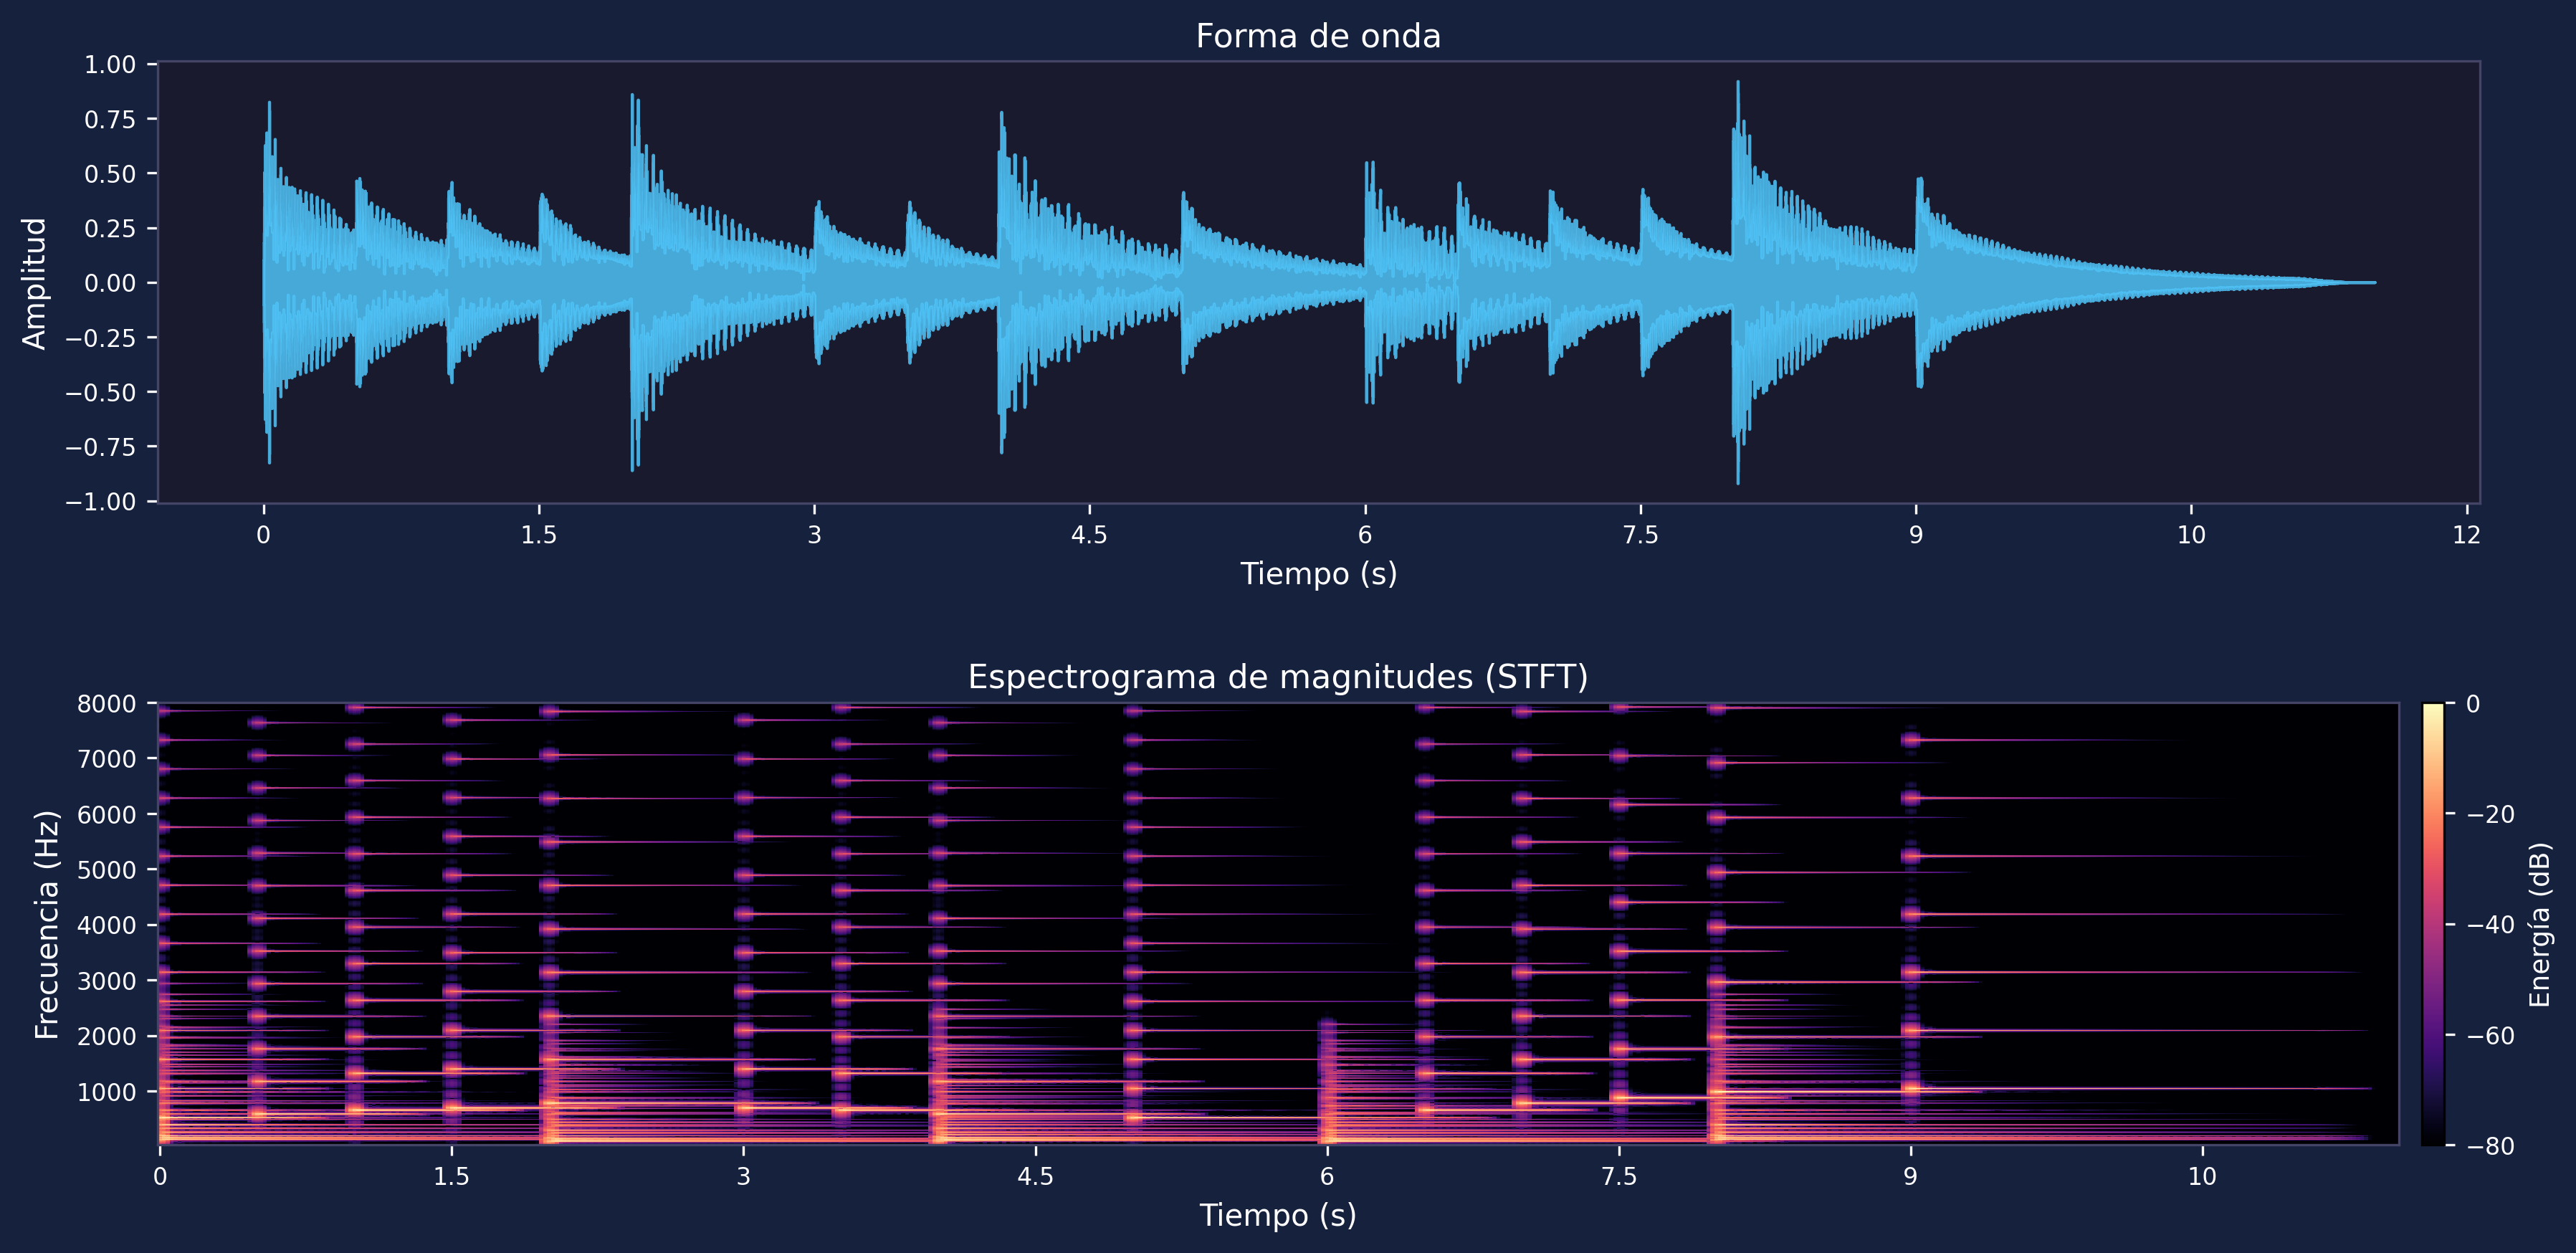
\includegraphics[width=\textwidth]{figs/stft_ejemplo.png}
    \caption{De la señal de audio al espectrograma. Superior: forma de
    onda de una grabación de piano. Inferior: espectrograma de magnitudes
    obtenido mediante la STFT. Las regiones más brillantes indican mayor
    energía espectral; los ataques de notas se aprecian como transitorios
    verticales de alta energía, y las notas sostenidas como bandas
    horizontales.}
    \label{fig:stft}
\end{figure}

El espectrograma proporciona una representación visual e intuitiva del
contenido musical: los ataques de notas aparecen como transitorios de
alta energía, las notas sostenidas como bandas horizontales, y los
acordes polifónicos como la superposición de múltiples bandas
frecuenciales simultáneas.

\subsection{El espectrograma Mel logarítmico}

El espectrograma lineal captura toda la información frecuencial de la
señal, pero no refleja la forma en que el ser humano percibe el sonido.
El sistema auditivo humano distingue con mayor precisión entre frecuencias
graves que entre frecuencias agudas de diferencia equivalente. Para
modelar esta percepción no lineal se introduce la \textit{escala Mel}
\cite{muller2021fundamentals}: una transformación que comprime las
frecuencias agudas y expande las graves, de modo que distancias iguales
en la escala Mel corresponden a intervalos percibidos como igualmente
separados por el oído humano.

En la práctica, esta transformación se implementa en dos pasos
sucesivos. Primero, un banco de filtros triangulares distribuidos
según la escala Mel agrupa la energía del espectrograma lineal en
bandas frecuenciales perceptualmente uniformes, produciendo el
espectrograma Mel (\textit{Mel spectrogram}). Segundo, se
aplica una compresión logarítmica sobre los valores de energía
resultantes, obteniendo el espectrograma Log-Mel
(\textit{Log-Mel spectrogram}): esta compresión reduce el rango
dinámico de la señal (que en una grabación de piano puede abarcar
varios órdenes de magnitud) y estabiliza la varianza de los datos
de entrada, facilitando la convergencia del proceso de aprendizaje
\cite{purwins2019deep}. La Figura~\ref{fig:logmel} ilustra el
resultado: las franjas de frecuencias agudas aparecen notablemente
más comprimidas que las graves, evidenciando la redistribución
perceptual característica de la escala Mel. 

\begin{figure}[htbp]
    \centering
    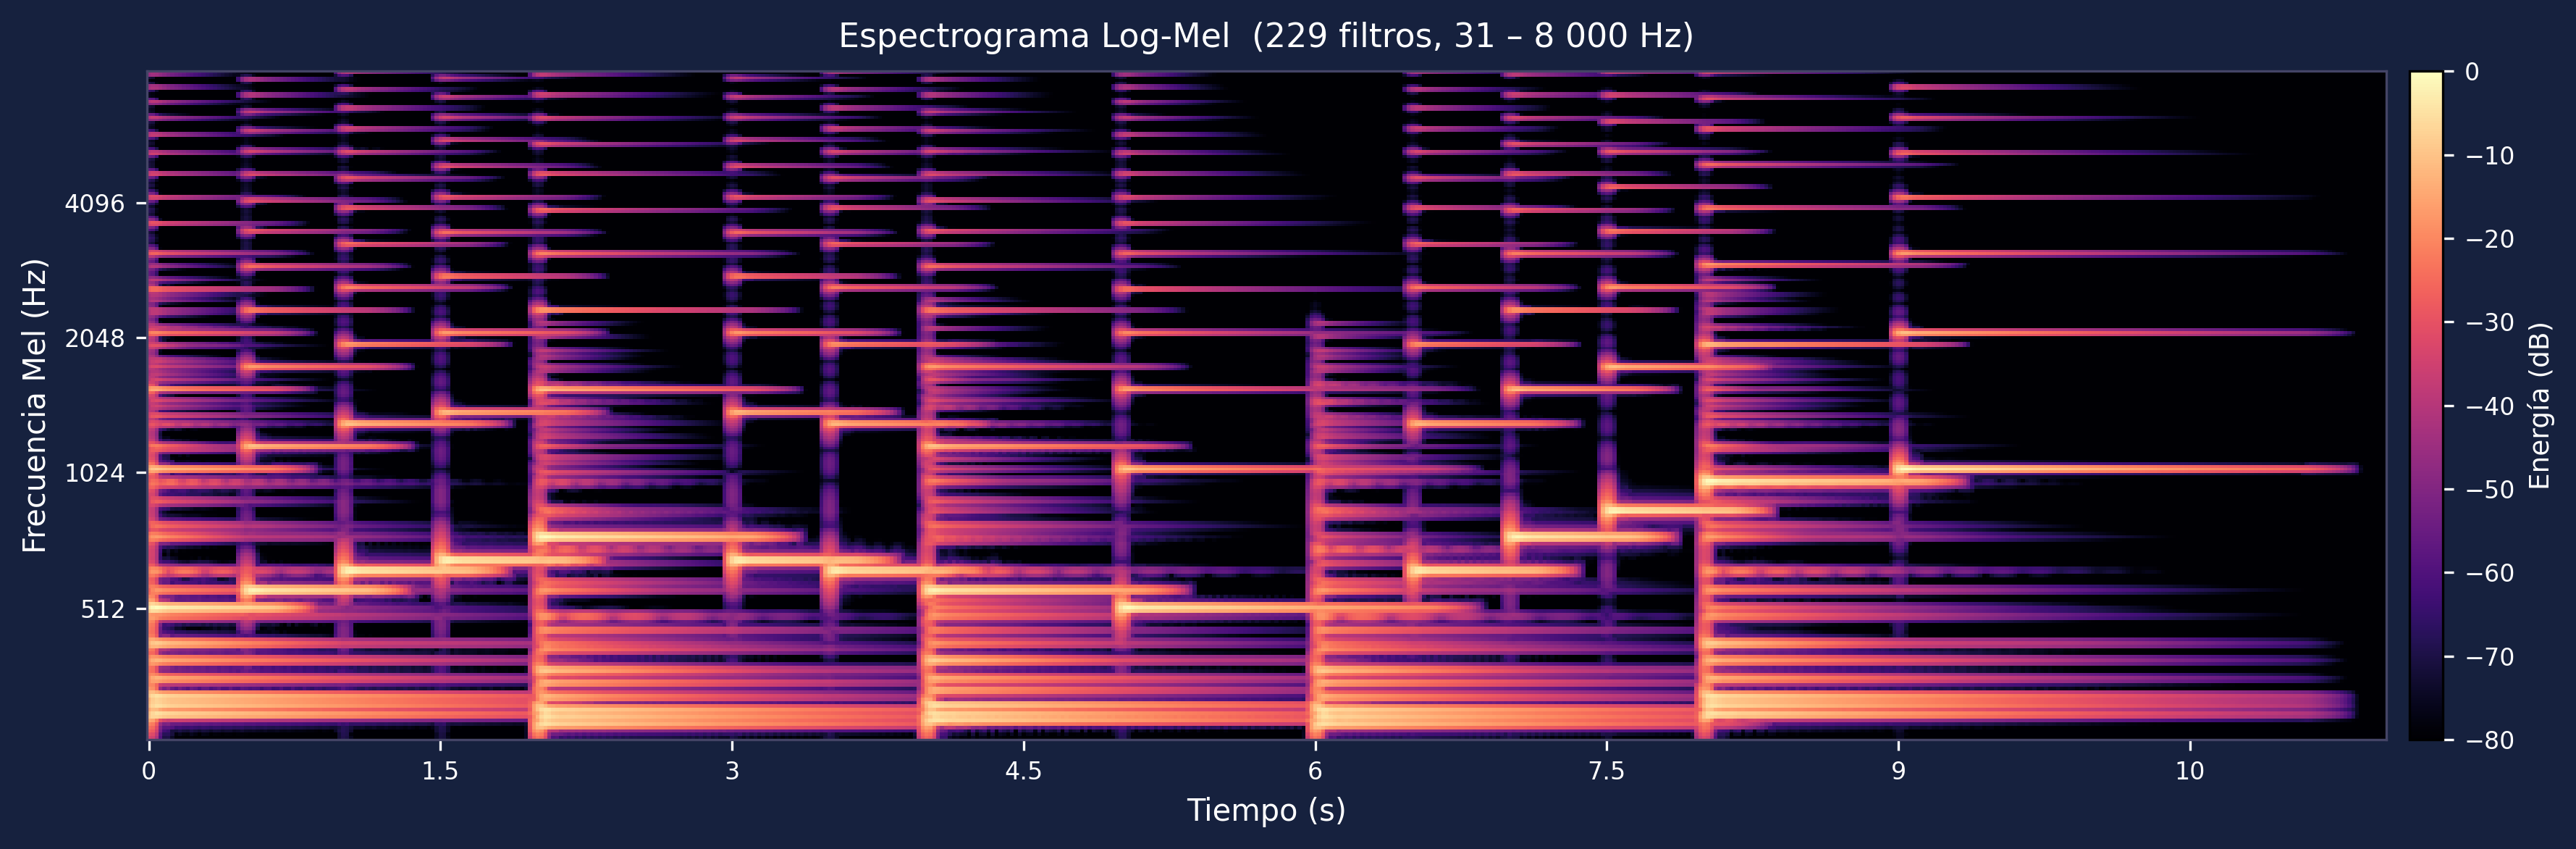
\includegraphics[width=\textwidth]{figs/logmel_ejemplo.png}
    \caption{Espectrograma Log-Mel de una interpretación de piano. En
    comparación con el espectrograma lineal, la escala Mel distribuye los
    filtros de forma más densa en las frecuencias graves —donde se
    concentra la mayor parte de la información armónica del piano— y más
    dispersa en las agudas, emulando la percepción auditiva humana.}
    \label{fig:logmel}
\end{figure}

El espectrograma Log-Mel se ha consolidado como la representación de
entrada estándar para tareas de análisis musical con redes neuronales
profundas \cite{purwins2019deep}, y es la adoptada en el sistema
desarrollado en este proyecto. Los parámetros concretos de su cálculo
se detallan en la Sección~\ref{sec:dominio_acustico}, junto con la
justificación de cada elección en el contexto de la transcripción de
piano.


% -----------------------------------------------------------
\section{Transcripción automática de música (AMT)}
\label{sec:amt}
% -----------------------------------------------------------

\subsection{Definición del problema}
 
La Transcripción Automática de Música (del inglés, \textit{Automatic Music Transcription}, en adelante AMT) puede definirse formalmente como el proceso computacional que,dada una señal de audio discreta $\mathbf{x} \in \mathbb{R}^{T}$,donde $T$ es el número de muestras de la señal, produce una representación simbólica estructurada $\mathcal{S}$ que describe los eventos musicales subyacentes que la componen \cite{benetos2019automatic}. Esta representación puede adoptar múltiples formas, siendo las más habituales el archivo MIDI (\textit{Musical Instrument Digital Interface}) y la partitura en notación estándar occidental o su equivalente digital en formato MusicXML.
 
Desde una perspectiva de aprendizaje automático, la AMT puede encuadrarse dentro
de las tareas de reconocimiento estructurado, en las que la salida no es una clase discreta singular, sino una secuencia de longitud variable de eventos interrelacionados. Cada evento musical queda caracterizado por cuatro atributos fundamentales: el tono (\textit{pitch}), que determina la frecuencia fundamental de la nota; el instante de inicio (\textit{onset}), que marca el momento exacto de la pulsación; la duración, que define el intervalo de
tiempo hasta la finalización del sonido (\textit{offset}); y la dinámica (\textit{velocity}),
que codifica la intensidad de la pulsación \cite{muller2021fundamentals}.
 
En el caso particular del piano, dominio exclusivo del presente proyecto, la complejidad
del problema se ve incrementada significativamente por varios factores acústicos inherentes
al instrumento. Su naturaleza intrínsecamente polifónica permite la pulsación simultánea
de hasta diez notas de forma independiente, provocando una superposición densa de
armónicos en el espectro de frecuencias que dificulta la separación de las fuentes sonoras
individuales. Adicionalmente, el uso del pedal de resonancia (\textit{sustain pedal})
extiende artificialmente la duración acústica de las notas, creando interferencias complejas
entre eventos musicales sucesivos. La amplia gama dinámica del instrumento, que abarca
desde el \textit{pianissimo} hasta el \textit{fortissimo}, introduce variaciones de hasta
cuatro órdenes de magnitud en la energía espectral de los ataques. Estos factores hacen
que la \textit{AMT} de piano siga siendo un problema abierto y un área de investigación
activa dentro del campo MIR \cite{benetos2019automatic}.
 
\subsection{Representaciones habituales}
 
La elección de las representaciones de los datos de entrada y salida constituye una
decisión de diseño fundamental en cualquier sistema de AMT, pues condiciona
directamente tanto la arquitectura del modelo como la naturaleza del aprendizaje supervisado.
 
En el dominio de la entrada acústica, las representaciones más habituales se derivan de la
Transformada de Fourier a Corto Plazo (\textit{Short-Time Fourier Transform}, STFT),
que permite analizar la evolución temporal del contenido frecuencial de la señal. A partir
del espectrograma de magnitudes resultante se han popularizado dos derivaciones
fundamentales: el espectrograma en escala Mel (\textit{Mel spectrogram}), que proyecta
las frecuencias lineales sobre una escala perceptualmente motivada que emula la respuesta
no lineal del sistema auditivo humano, y su versión logarítmica (\textit{Log-Mel
spectrogram}), que comprime adicionalmente el rango dinámico y ha demostrado
empíricamente ser la representación de referencia para tareas de análisis musical con
redes neuronales profundas \cite{purwins2019deep}. Esta última es la adoptada en el
presente trabajo, tal y como se detalla en la Sección~\ref{sec:dominio_acustico}.
 
En lo que respecta a la representación de salida, conviene distinguir entre el enfoque histórico y el moderno, para entender la elección en este proyecto. El formato más extendido históricamente ha sido el \textit{piano-roll}: una representación bidimensional discreta en la que el eje horizontal codifica el tiempo (segmentado en tramas de
duración fija) y el eje vertical los 88 semitonos del piano, tal y como se muestra en la figura ~\ref{fig:piano_roll}, de modo que cada celda activa indica la presencia de una nota en ese instante
\cite{benetos2019automatic}. Aunque intuitiva, esta representación acopla rígidamente la resolución temporal a la granularidad de la
trama, limitando la expresividad de los atributos dinámicos y de duración. Los enfoques más recientes han evolucionado hacia representaciones basadas en eventos discretos: la salida es una secuencia de unidades simbólicas denominadas \textit{tokens}, cada una de las cuales codifica un evento musical específico: la activación de una nota (\textit{Note-On}), su desactivación (\textit{Note-Off}) o un desplazamiento temporal (\textit{Time-Shift}), eliminando así la dependencia de la trama fija \cite{oore2020time}. Es esta segunda representación la adoptada en el sistema desarrollado en este proyecto, cuyo vocabulario se describe en detalle en la Sección~\ref{sec:dominio_simbolico}.

\begin{figure}[htbp]
    \centering
    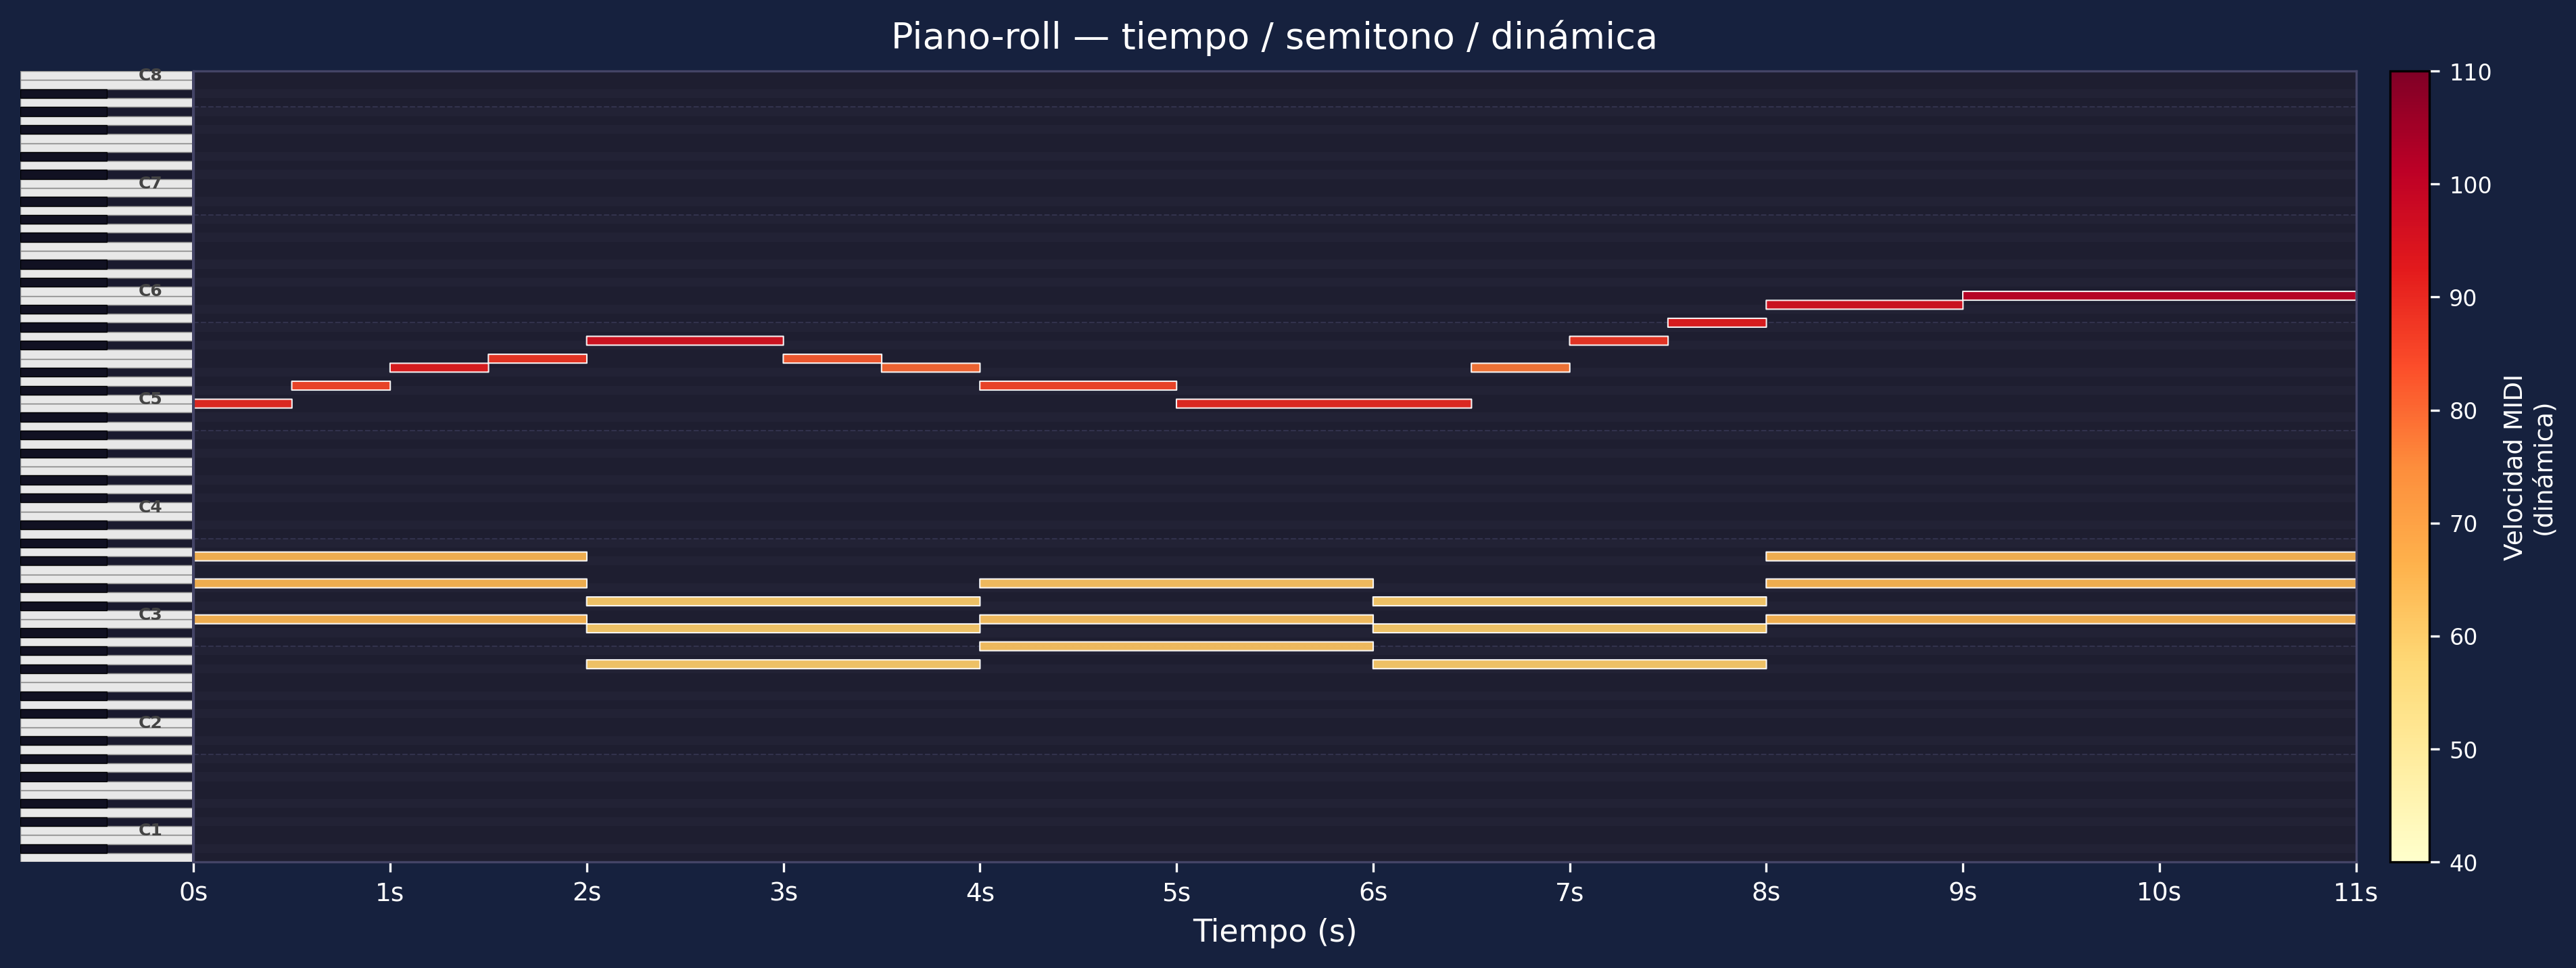
\includegraphics[width=0.85\textwidth]{figs/piano_roll_ejemplo.png}
    \caption{Ejemplo de representación \textit{piano-roll}: el eje
    horizontal codifica el tiempo y el eje vertical los 88 semitonos
    del piano. Cada rectángulo representa una nota activa, con su duración y dinámica codificadas visualmente.}
    \label{fig:piano_roll}
\end{figure}
 
% -----------------------------------------------------------
\section{Enfoques clásicos basados en \textit{frames}}
% -----------------------------------------------------------
 
\subsection{Clasificación por \textit{frames} y \textit{piano-roll}}
 
Durante la primera generación de sistemas de AMT basados en aprendizaje
automático, el paradigma dominante fue la clasificación independiente por tramas
(\textit{frame-level classification}). En este enfoque, el modelo procesa una ventana de
audio de duración fija (típicamente entre 20 y 100 milisegundos) y produce, para cada
trama, un vector binario de 88 dimensiones que indica el estado de activación de cada tecla del piano en ese instante concreto \cite{benetos2019automatic}. La concatenación
temporal de estos vectores genera la representación \textit{piano-roll}, que posteriormente es procesada mediante heurísticas de post-procesado para agrupar activaciones consecutivas y extraer las notas completas con sus atributos de duración y velocidad.
 
Las arquitecturas empleadas en esta etapa fueron esencialmente Redes Neuronales
Convolucionales (\textit{Convolutional Neural Networks}, CNN), que demostraron ser
altamente eficaces para la extracción de características locales en el espectrograma, tales como la detección de ataques transitorios y la identificación de estructuras armónicas periódicas. Trabajos seminales como el de Sigtia et al.\ \cite{sigtia2016end} combinaron estas CNN con Redes Neuronales Recurrentes (\textit{Recurrent Neural Networks}, RNN) para incorporar dependencias temporales a corto plazo, sentando las bases de la arquitectura híbrida CNN-RNN que dominó la disciplina durante varios años.
En esta misma línea, Kong et al.\ \cite{kong2021high} demostraron que modelos de
clasificación por frames entrenados con pérdidas específicamente diseñadas para la
detección de \textit{onsets} podían alcanzar rendimientos competitivos sobre el
\textit{dataset} MAESTRO, obteniendo rendimientos de predicción superiores al 96\% bajo
condiciones de evaluación estándar.
 
\subsection{Limitaciones}
 
A pesar de los resultados destacables que los enfoques basados en \textit{frames} han
logrado, presentan limitaciones estructurales que restringen su capacidad de modelado y
que motivan directamente la propuesta del presente trabajo.
 
La limitación más fundamental es la suposición implícita de independencia entre tramas.
Al clasificar cada ventana temporal de forma aislada, estos modelos no disponen de
mecanismo alguno para razonar sobre la estructura musical global de una pieza: no pueden
capturar dependencias armónicas a largo plazo, ni modelar correctamente el arco expresivo
de una frase musical, ni anticipar la resolución de una disonancia. Esta miopía temporal
limita especialmente la precisión en la detección de \textit{offsets}, ya que la finalización
de una nota depende frecuentemente de su contexto melódico y de la interacción con el
pedal \cite{benetos2019automatic}.
 
Una segunda limitación inherente es la dificultad para modelar de forma conjunta todos
los atributos de una nota. La formulación como clasificación binaria en cada trama obliga
a tratar el \textit{pitch}, la duración y la velocidad como variables independientes,
requiriendo etapas de post-procesado para obtener los eventos completos. Este
desacoplamiento introduce errores de propagación que se acumulan a lo largo de la pieza,
especialmente en pasajes con alta densidad polifónica. Finalmente, la dependencia de una
resolución temporal fija de la trama impone un compromiso entre resolución temporal y
coste computacional que no puede ajustarse dinámicamente en función de la densidad
musical local.
 
% -----------------------------------------------------------
\section{Modelos de secuencia a secuencia y generación de eventos}
\label{sec:seq2seq}
% -----------------------------------------------------------

\subsection{Audio a secuencia de \textit{tokens}}

Para superar las limitaciones de los enfoques basados en \textit{frames},
la comunidad investigadora en MIR ha explorado de forma creciente la
reformulación de la AMT como un problema de traducción de secuencia a
secuencia. En este paradigma,
el sistema aprende un mapeo directo desde una representación continua de
la señal acústica hacia una secuencia discreta de \textit{tokens} que
codifican los eventos musicales, de manera análoga a la traducción
automática en el procesamiento del lenguaje natural
(\textit{Natural Language Processing}, NLP) \cite{oore2020time}.

El diseño del vocabulario de \textit{tokens} es un componente central
de este enfoque. La representación de eventos propuesta originalmente
por Oore et al.\ \cite{oore2020time} codifica la música de piano
mediante cuatro tipos de eventos:

\begin{itemize}
    \item \textit{NOTE\_ON}$(p)$: activa la nota de tono $p$.
    \item \textit{NOTE\_OFF}$(p)$: desactiva la nota de tono $p$.
    \item \textit{TIME\_SHIFT}$(t)$: avanza el cursor temporal $t$
          unidades de tiempo.
    \item \textit{SET\_VELOCITY}$(v)$: establece la intensidad de la nota.
\end{itemize}

Esta gramática de eventos permite representar de forma compacta y sin
pérdida de información cualquier pieza de piano con polifonía arbitraria,
eliminando la dependencia de la trama fija y codificando de manera
integral los cuatro atributos musicales fundamentales en una única
secuencia lineal. El vocabulario implementado en el presente trabajo,
descrito en la Sección~\ref{sec:dominio_simbolico}, sigue esta misma
filosofía con adaptaciones específicas en la cuantización de la velocidad
y la resolución temporal.

\subsection{El Transformer en el paradigma Seq2Seq}

La arquitectura Transformer \cite{vaswani2017attention} ha demostrado
ser especialmente adecuada para el modelado de la AMT en el paradigma
Seq2Seq, gracias a su capacidad para capturar dependencias a largo plazo
mediante el mecanismo de autoatención. La resolución correcta de la
armonía, la coherencia rítmica y la continuidad del fraseo requieren que
el modelo pueda relacionar eventos separados por varios compases, algo
que las RNN no logran eficientemente. La arquitectura, su mecanismo
interno y su configuración Encoder-Decoder se describen en detalle en la
Sección~\ref{sec:transformer}.


% -----------------------------------------------------------
\section{La arquitectura Transformer}
\label{sec:transformer}
% -----------------------------------------------------------

La arquitectura Transformer \cite{vaswani2017attention} ha supuesto un
cambio de paradigma en el procesamiento de secuencias, desplazando a las
redes recurrentes como estándar de referencia en múltiples dominios. A
diferencia de las RNN, que procesan la secuencia elemento a elemento de
forma estrictamente secuencial, el Transformer procesa todos los elementos
en paralelo, capturando de forma directa las dependencias entre posiciones
lejanas. Esta característica lo convierte en una herramienta especialmente
adecuada para el dominio musical, donde la comprensión de una nota puede
requerir relacionarla con eventos separados por varios compases.

% -----------------------------------------------------------
\subsection{El mecanismo de autoatención}
% -----------------------------------------------------------

El componente central del Transformer es el mecanismo de
\textit{autoatención} (\textit{self-attention}), que permite a cada
elemento de una secuencia determinar dinámicamente qué otros elementos
son relevantes para su propia representación \cite{vaswani2017attention}.

Intuitivamente, el mecanismo puede entenderse así: para cada elemento,
el modelo formula una \textit{consulta} (\textit{query}) que expresa qué
información necesita; al mismo tiempo, cada elemento publica una
\textit{clave} (\textit{key}) que describe qué información ofrece y un
\textit{valor} (\textit{value}) que contiene esa información. La atención
que el elemento $i$ presta al elemento $j$ se determina midiendo la
similitud entre la consulta de $i$ y la clave de $j$: cuanto mayor sea
la similitud, mayor será la ponderación del valor de $j$ en la
representación actualizada de $i$.

Formalmente, dados los tensores de consultas $\mathbf{Q}$, claves
$\mathbf{K}$ y valores $\mathbf{V}$, la atención se calcula como:

\begin{equation}
    \text{Attention}(\mathbf{Q}, \mathbf{K}, \mathbf{V}) =
    \text{softmax}\!\left(
    \frac{\mathbf{Q}\mathbf{K}^{\top}}{\sqrt{d_k}}
    \right)\mathbf{V}
    \label{eq:attention}
\end{equation}

donde $d_k$ es la dimensión de las claves y el factor $\sqrt{d_k}$ escala
los productos internos para estabilizar los gradientes durante el
entrenamiento. El resultado es una nueva representación de cada elemento
que integra, de forma ponderada, la información de todos los demás
elementos de la secuencia.

Para capturar relaciones de distinta naturaleza de forma simultánea, el
Transformer emplea la \textit{atención multi-cabeza}
(\textit{Multi-Head Attention}): el mecanismo de atención se aplica en
paralelo varias veces, con proyecciones lineales independientes para cada
cabeza. Las salidas de todas las cabezas se concatenan y se proyectan a
la dimensión original, enriqueciendo la capacidad representacional del
modelo \cite{vaswani2017attention}.

% -----------------------------------------------------------
\subsection{Codificación posicional}
% -----------------------------------------------------------

A diferencia de las redes recurrentes, el Transformer no posee una
noción inherente del orden de los elementos en la secuencia: el mecanismo
de atención trata todos los pares de posiciones de forma simétrica. Para
dotar al modelo de información sobre la posición de cada elemento, se
suma a su representación una \textit{codificación posicional}
(\textit{positional encoding}) \cite{vaswani2017attention}.

La formulación original utiliza funciones sinusoidales de distinta
frecuencia para cada dimensión del espacio de representación, de forma
que cada posición recibe un vector único e interpretable por el modelo.
Una alternativa es aprender las codificaciones posicionales directamente
de los datos, lo que permite adaptar la representación posicional a las
particularidades del dominio \cite{dosovitskiy2021image}. La elección
entre ambas estrategias tiene implicaciones sobre la capacidad del modelo
para generalizar a secuencias de longitud no vista durante el
entrenamiento, aspecto especialmente relevante al procesar piezas
musicales de duración variable.

% -----------------------------------------------------------
\subsection{Configuración Encoder-Decoder}
% -----------------------------------------------------------

Para tareas de traducción de secuencias en las que entrada y salida son
de distinta naturaleza y longitud, el Transformer adopta una configuración
\textit{Encoder-Decoder} \cite{vaswani2017attention}, ilustrada en la
Figura~\ref{fig:encoder_decoder}.

El \textit{codificador} (\textit{encoder}) recibe la secuencia de entrada
completa y la procesa mediante capas sucesivas de autoatención y redes de
propagación hacia adelante (\textit{feed-forward networks}), produciendo
una secuencia de representaciones contextualizadas que capturan las
relaciones globales entre todos los elementos de la entrada.

El \textit{decodificador} (\textit{decoder}) genera la secuencia de
salida de forma \textit{autorregresiva}: produce un elemento en cada
paso, condicionado tanto a las representaciones del codificador como a
todos los elementos ya generados. Para acceder a la información del
codificador, cada capa del decodificador incorpora un mecanismo de
\textit{atención cruzada} (\textit{cross-attention}), donde las consultas
provienen del decodificador y las claves y valores del codificador. Para
garantizar que la predicción de cada elemento dependa únicamente de los
anteriores, la autoatención del decodificador aplica una \textit{máscara
causal} que impide el acceso a posiciones futuras de la secuencia.

\begin{figure}[htbp]
    \centering
    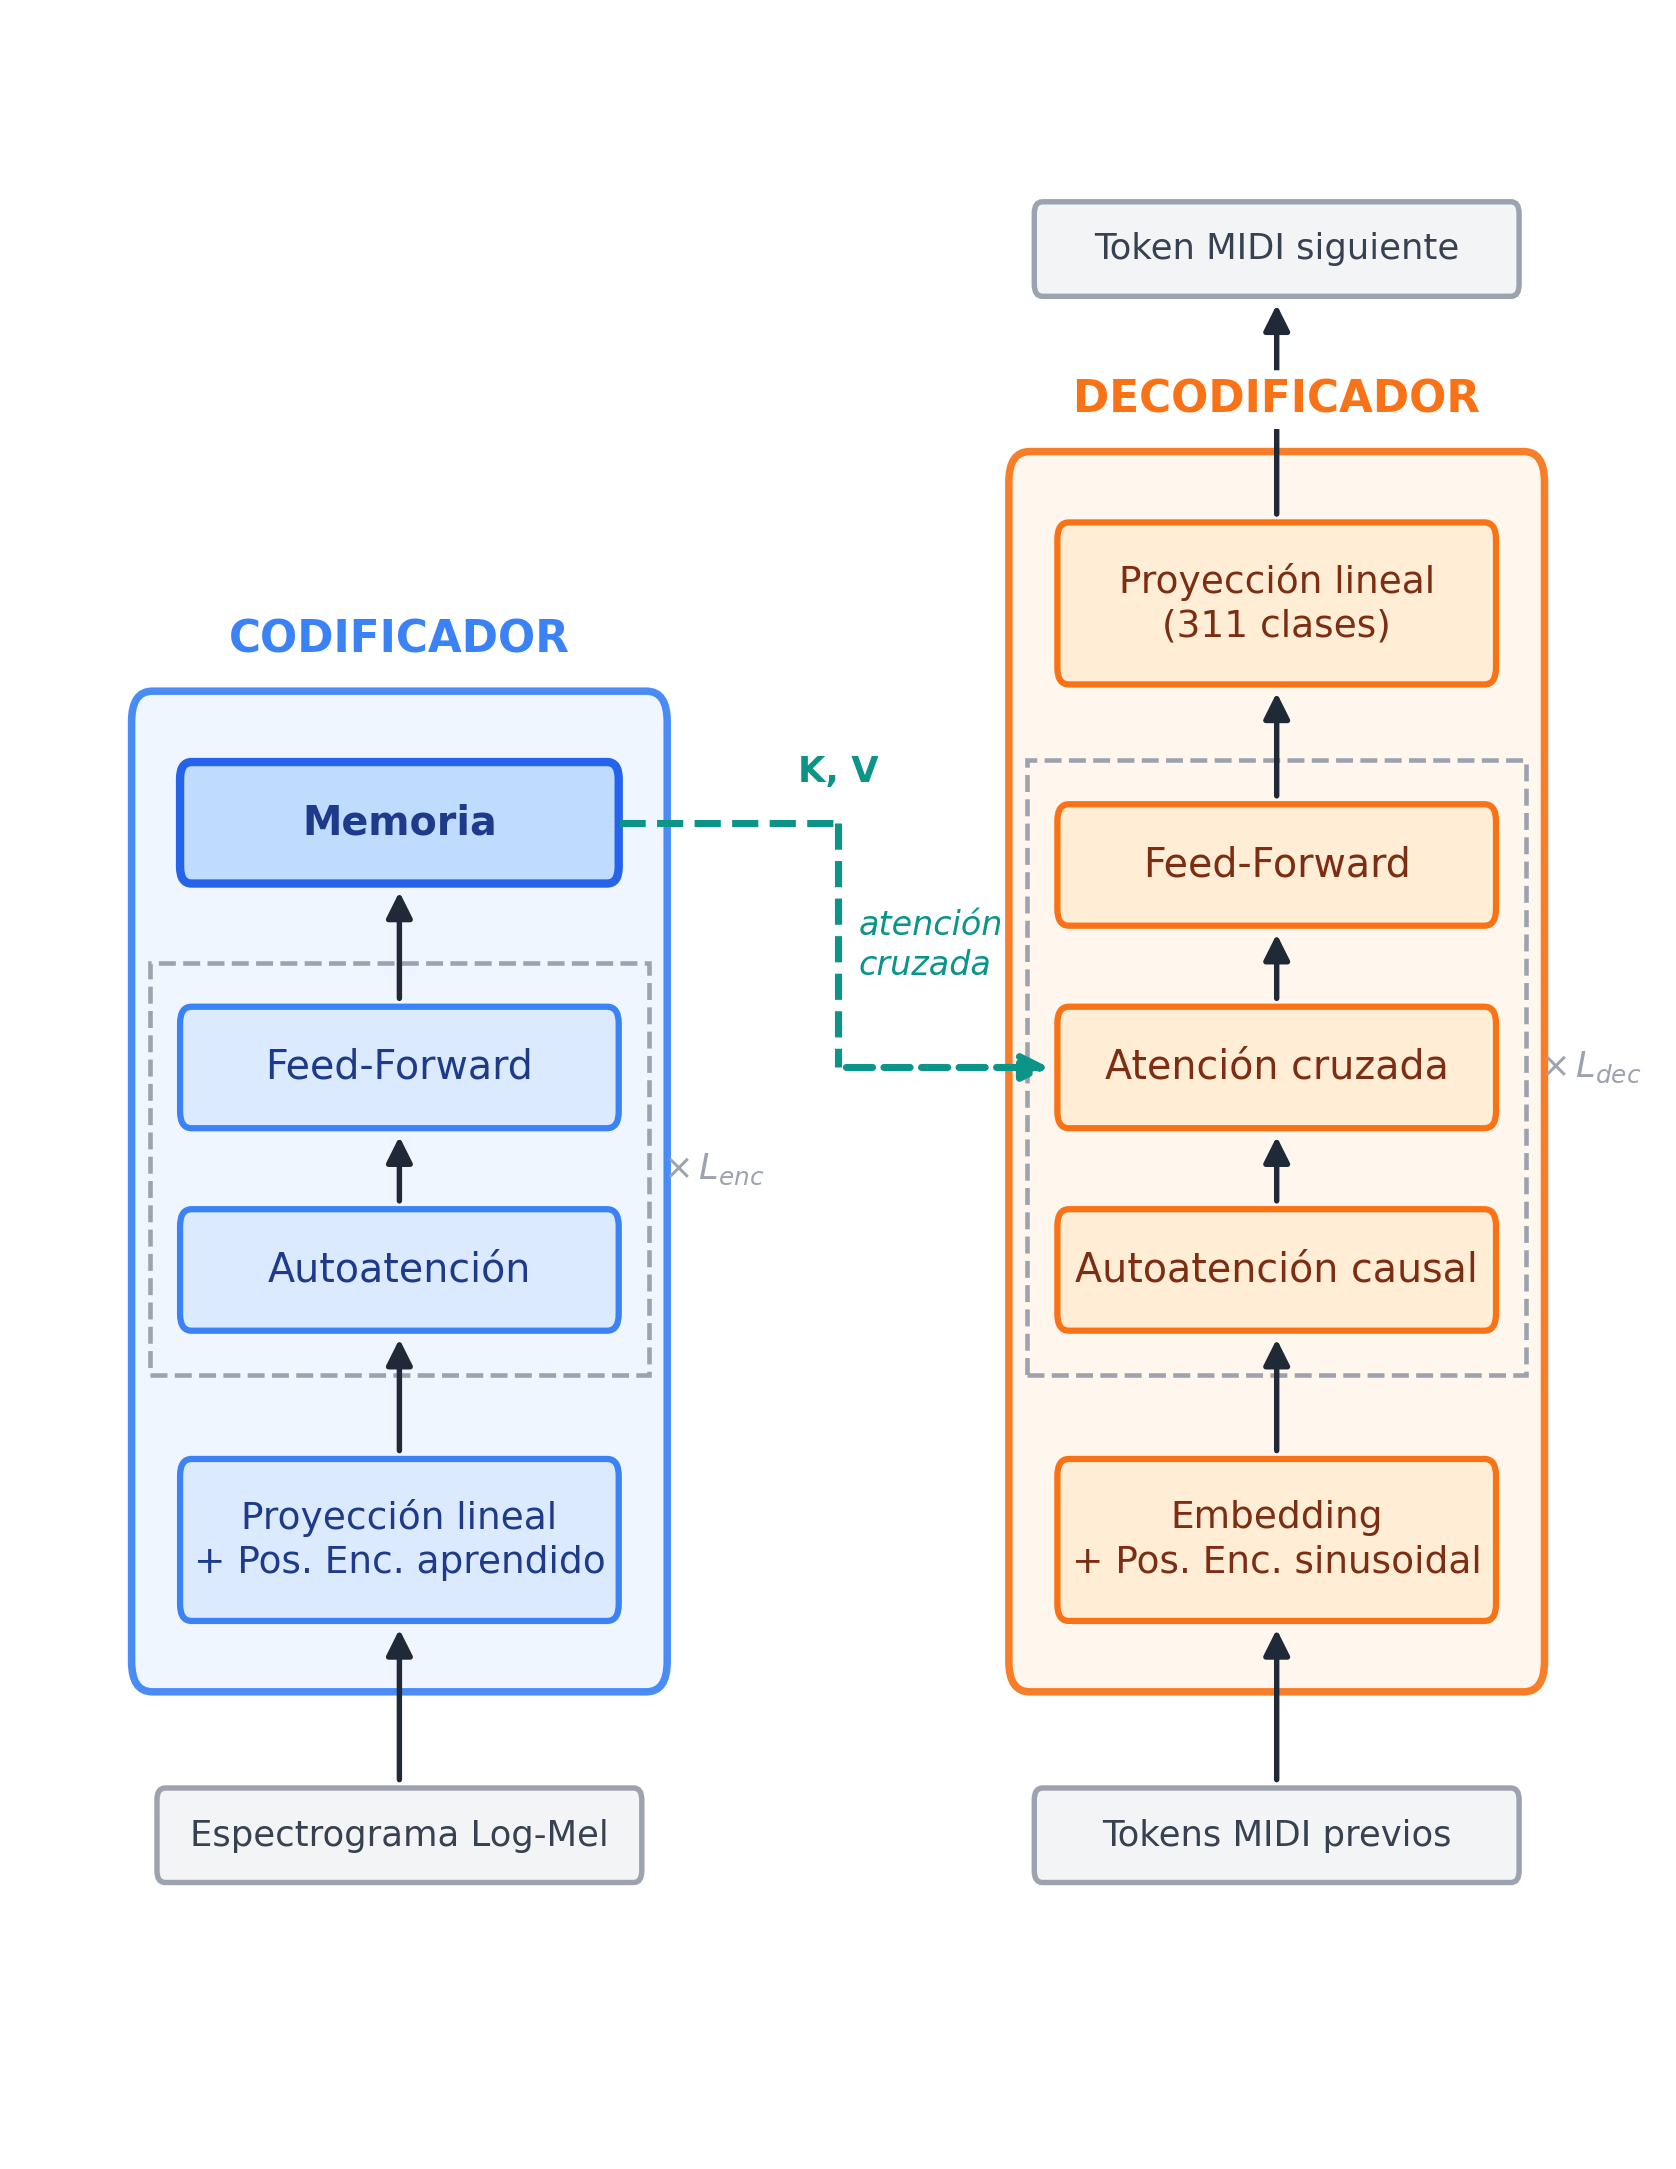
\includegraphics[width=0.85\textwidth]{figs/encoder_decoder.png}
    \caption{Configuración \textit{Encoder-Decoder} del Transformer
    \cite{vaswani2017attention}. Las entradas y salidas (en gris) se
    procesan fuera de los bloques principales. El codificador produce
    la \textit{Memoria}, de la que el decodificador extrae claves
    ($\mathbf{K}$) y valores ($\mathbf{V}$) mediante atención cruzada
    en cada una de sus $L_{\mathrm{dec}}$ capas. Las cajas punteadas
    delimitan los bloques que se apilan $L$ veces.}
    \label{fig:encoder_decoder}
\end{figure}

% -----------------------------------------------------------
\subsection{Aplicación al problema de la AMT}
% -----------------------------------------------------------

Esta configuración resulta especialmente adecuada para la transcripción
automática de música. El codificador procesa la representación acústica
de la pieza (el espectrograma Log-Mel descrito en la
Sección~\ref{sec:representacion_audio}) y el decodificador genera la
secuencia de eventos musicales simbólicos que la describe. La generación
autorregresiva garantiza la coherencia de la secuencia de salida: cada
evento MIDI predicho puede condicionar el siguiente, de manera análoga
a la traducción automática en el procesamiento del lenguaje natural.

La ventaja fundamental del Transformer frente a los enfoques clásicos es
su capacidad para modelar dependencias a largo plazo
\cite{vaswani2017attention}. En el dominio musical, esto resulta crítico:
la correcta interpretación de un acorde puede depender del contexto
armónico establecido varios compases antes, y la resonancia producida por
el pedal de sustain puede solapar notas separadas por varios segundos. El
mecanismo de autoatención accede directamente a cualquier posición de la
secuencia de entrada sin la degradación de información que afecta a las
redes recurrentes en dependencias muy extendidas.
 
% -----------------------------------------------------------
\section{Atención eficiente y dispersa}
% -----------------------------------------------------------

\subsection{Coste cuadrático de la autoatención}

A pesar de sus ventajas en el modelado de dependencias globales, la
arquitectura Transformer estándar presenta una limitación computacional
crítica cuando se aplica al dominio del audio continuo. El cálculo de la
autoatención sobre una secuencia de $N$ \textit{tokens} requiere
construir y operar con una matriz de atención de dimensiones $N \times N$,
lo que conlleva una complejidad temporal y espacial de
$\mathcal{O}(N^2)$ \cite{vaswani2017attention}. En el dominio del
procesamiento del lenguaje natural, donde $N$ raramente supera los miles
de \textit{tokens}, este coste resulta asumible. Sin embargo, en el
dominio del audio musical, la situación es radicalmente diferente.

Para ilustrar la magnitud del problema en el contexto concreto de este
proyecto: con los parámetros de espectrograma definidos en la
Sección~\ref{sec:dominio_acustico}, frecuencia de muestreo
$f_s = 16000\,\mathrm{Hz}$ y un \textit{hop size} de 320 muestras
(el desplazamiento entre ventanas de análisis consecutivas), cada
segundo de audio genera $16000 / 320 = 50$ tramas espectrales. Una
pieza musical de cinco minutos de duración, representativa del corpus
MAESTRO, produce por tanto $N = 15000$ tramas. Aplicar autoatención
estándar sobre esta secuencia requeriría almacenar una matriz de
$15000 \times 15000 = 225 \times 10^6$ valores de atención, con un
consumo de memoria que, para precisión de coma flotante de 32 bits,
asciende a aproximadamente 900\,MB únicamente para la capa de atención.
Dado que los modelos profundos apilan múltiples capas de atención y que
el entrenamiento requiere almacenar los gradientes intermedios, este
coste resulta prohibitivo incluso para hardware de cómputo especializado
de alta gama.

\subsection{Ventanas deslizantes frente a dispersidad dinámica}

Para mitigar el cuello de botella cuadrático, se han propuesto en la
literatura diversas estrategias de atención eficiente que reducen el
número de pares de posiciones que se atienden mutuamente, restringiendo
la conectividad de la matriz de atención de forma controlada
\cite{tay2020efficient}.

Un primer grupo de métodos emplea patrones de conectividad fija definidos
a priori, independientemente del contenido de la secuencia. El mecanismo
de atención por ventana deslizante (\textit{Sliding Window Attention})
es el representante más destacado de esta familia: cada posición $i$
únicamente atiende a las posiciones comprendidas en un intervalo
$[i - w,\, i + w]$, donde $w$ es el tamaño de ventana, reduciendo la
complejidad a $\mathcal{O}(N \cdot w)$ \cite{beltagy2020longformer}. Este
enfoque es computacionalmente eficiente y estructuralmente sencillo, y
resulta especialmente apropiado en dominios en los que las dependencias
relevantes son predominantemente locales. En el dominio del audio musical,
la coherencia acústica a muy corto plazo (como la evolución de un
armónico o el transitorio de un ataque) se captura eficazmente mediante
ventanas locales. Sin embargo, la atención por ventana deslizante
sacrifica por diseño la capacidad de modelar dependencias globales: un
acorde en el compás diez no puede influir directamente en la predicción
del compás uno si ambos quedan fuera del radio de la ventana.

Un segundo grupo de métodos, conceptualmente más ambicioso, adopta un
enfoque de dispersidad dinámica o aprendida (\textit{dynamic sparse
attention}): en lugar de definir a priori qué posiciones se atienden
entre sí, el modelo aprende a seleccionar, en función del contenido de
la secuencia, las conexiones más relevantes para cada instancia concreta
\cite{child2019generating}. El modelo \textit{Sparse Transformer}
propuesto por Child et al.\ \cite{child2019generating} demostró que
restringir la autoatención a un subconjunto aprendido de conexiones, combinando patrones locales y globales de forma estocástica, permitía procesar secuencias de hasta 12288 \textit{tokens} manteniendo
una calidad generativa comparable a la atención completa. En esta misma
línea de investigación, el modelo \textit{BigBird} de Zaheer et al.\
\cite{zaheer2020big} formalizó teóricamente las garantías de
expresividad de los Transformers dispersos, demostrando que la
combinación de atención local por ventana, atención global sobre un
conjunto reducido de \textit{tokens} de resumen y atención aleatoria es
suficiente para aproximar cualquier función computable por un Transformer
denso.

La arquitectura Sparsifiner \cite{wei2023sparsifiner}, que sirve de
inspiración directa para el mecanismo de atención implementado en este
proyecto, extiende este paradigma al dominio de la visión por computador,
interpretando los \textit{tokens} de entrada como parches de una imagen
bidimensional y aprendiendo a construir de forma dinámica e
instancia-dependiente un grafo de conectividad dispersa sobre dichos
parches. Esta perspectiva resulta especialmente pertinente para el dominio
del espectrograma de audio, que puede interpretarse conceptualmente como
una imagen bidimensional en el plano tiempo-frecuencia: las regiones
espectralmente activas, como ataques de notas, transitorios o armónicos
prominentes, concentran la mayor densidad de información relevante para
la transcripción, mientras que las regiones de silencio o contenido
acústico estacionario presentan información redundante y de baja
varianza. Frente a la \textit{Sliding Window Attention}, que restringe la
conectividad de forma fija e independiente del contenido, Sparsifiner
selecciona dinámicamente qué dependencias son relevantes para cada
instancia concreta, lo que lo convierte en la estrategia de atención
eficiente adoptada en el codificador del presente sistema. Su adaptación
al dominio del espectrograma musical se describe en detalle en el
Capítulo~\ref{cap:arquitectura}.


% -----------------------------------------------------------
\section{Métricas de evaluación en AMT}
\label{sec:metricas}
% -----------------------------------------------------------

La evaluación objetiva de un sistema de AMT requiere métricas que
permitan comparar la secuencia de eventos predicha con la verdad base
de forma reproducible y comparable con el estado del arte. En este campo
coexisten dos paradigmas de evaluación con objetivos complementarios
\cite{benetos2019automatic}.

\subsection{Evaluación a nivel de trama}

El enfoque más sencillo compara el estado de activación de cada nota en
cada instante de tiempo, evaluando si el conjunto de notas activas en una
trama predicha coincide con el de la trama de referencia. Para cada
trama, se calcula el número de verdaderos positivos (notas activas en
ambas secuencias), falsos positivos (activas solo en la predicción) y
falsos negativos (activas solo en la referencia). A partir de estos
valores se derivan la \textit{precisión} $P$, la \textit{exhaustividad}
$R$ y el \textit{F1-score}:

\begin{equation}
    P = \frac{TP}{TP + FP}, \qquad
    R = \frac{TP}{TP + FN}, \qquad
    F1 = \frac{2 \cdot P \cdot R}{P + R}
    \label{eq:f1}
\end{equation}

Aunque computacionalmente sencilla, la evaluación por tramas presenta
una limitación fundamental: al no modelar explícitamente los eventos de
inicio y fin de cada nota, sobrevalora sistemas que predicen
correctamente la presencia de una nota pero con duración incorrecta.

\subsection{Evaluación a nivel de nota}

Para una evaluación más rigurosa, el paradigma estándar en la literatura
AMT compara las notas como eventos completos, caracterizados por su tono,
instante de inicio (\textit{onset}) e instante de fin (\textit{offset})
\cite{benetos2019automatic}. Una nota predicha se considera un verdadero
positivo si satisface simultáneamente dos condiciones: el tono coincide
exactamente con el de la nota de referencia, y su \textit{onset} se
encuentra dentro de una ventana de tolerancia de $\pm 50\,\mathrm{ms}$
respecto al \textit{onset} de referencia. Para la evaluación con
\textit{offset}, se exige adicionalmente que el \textit{offset} predicho
se encuentre dentro de $\pm 50\,\mathrm{ms}$ o del $20\,\%$ de la
duración de la nota de referencia, el que sea mayor
\cite{muller2021fundamentals}.

Esta familia de métricas se desglosa en tres variantes complementarias:
evaluación de \textit{onset} únicamente, que mide la capacidad del
modelo para detectar el inicio de cada nota; evaluación de
\textit{onset} con \textit{offset}, que añade la exigencia de
transcribir correctamente la duración; y evaluación de \textit{onset}
con velocidad, que valora conjuntamente la detección del ataque y la
fidelidad dinámica de la interpretación. Esta combinación permite
diagnosticar de forma independiente los distintos aspectos de la
transcripción sin recurrir a una métrica única excesivamente
penalizadora para un sistema en fase experimental. El protocolo de
evaluación concreto aplicado sobre el conjunto de prueba de MAESTRO
se detalla en el Capítulo~\ref{cap:resultados}.

\subsection{Herramienta de evaluación: \texttt{mir\_eval}}

El cálculo de todas estas métricas se realiza mediante la biblioteca
\texttt{mir\_eval}, que proporciona una implementación de referencia
transparente y reproducible de los estándares de evaluación en
Recuperación de Información Musical. Su uso garantiza que los resultados
obtenidos son directamente comparables con los publicados en la
literatura, eliminando ambigüedades en la definición de las ventanas de
tolerancia y en el proceso de emparejamiento entre notas predichas y de
referencia.


% -----------------------------------------------------------
\section{Resumen y posicionamiento del trabajo}
% -----------------------------------------------------------
 
La revisión del estado del arte presentada en este capítulo permite identificar con claridad
la trayectoria evolutiva de la AMT y situar la propuesta del presente proyecto dentro
de ella. Los enfoques clásicos basados en clasificación por \textit{frames} sentaron las
bases metodológicas de la disciplina y alcanzaron rendimientos notables en condiciones
controladas, pero su incapacidad estructural para modelar dependencias temporales a
largo plazo y su tratamiento desacoplado de los atributos musicales constituyen limitaciones
difícilmente superables dentro de ese paradigma.
 
La irrupción de la arquitectura Transformer y su aplicación al problema de la AMT
como traducción de secuencia a secuencia ha abierto una vía de investigación
cualitativamente diferente, en la que el modelo aprende de forma integral y conjunta todos
los atributos de los eventos musicales, capturando dependencias globales gracias al
mecanismo de autoatención. No obstante, el coste computacional cuadrático $\mathcal{O}(N^2)$
de la atención estándar constituye un obstáculo significativo para su aplicación a señales
de audio de larga duración, que es precisamente el caso de las interpretaciones de piano
presentes en el corpus MAESTRO.
 
El presente Trabajo Fin de Grado se posiciona en la intersección de estas dos líneas de
investigación. Se formula la AMT de piano polifónico como un problema de
traducción de secuencia a secuencia, empleando un vocabulario basado en eventos
MIDI de 311 \textit{tokens}. Para abordar el cuello de botella computacional de la
autoatención estándar, se adopta como mecanismo central del codificador la atención
dispersa instancia-dependiente propuesta por Sparsifiner \cite{wei2023sparsifiner}: en
lugar de restringir la conectividad mediante una ventana local fija, como haría la
\textit{Sliding Window Attention}, el modelo aprende a construir dinámicamente el grafo
de atención en función del contenido espectral de cada fragmento de audio, seleccionando
exclusivamente las dependencias temporales más informativas para la transcripción. Esta
elección permite mantener la capacidad de capturar dependencias a largo plazo, esencial
para modelar la armonía y el fraseo musical, mientras se reduce el coste efectivo de
atención a $\mathcal{O}(r_{attn} \cdot T^2)$ con $r_{attn} = 0.25$. La implementación
de este mecanismo, incluyendo las adaptaciones necesarias para el dominio del audio de
longitud variable, se detalla en el Capítulo~\ref{cap:arquitectura}.